
% manual maniFEM

\def\manifemversion{21.04}
\def\manualversion{21.05}

\magnification\magstep1
\nopagenumbers
\pretolerance=1200
\overfullrule=0pt 
\spaceskip=0.3333em plus 1.5pt minus 0.3pt
\xspaceskip=0.5em plus 2pt minus 0.5pt

% Plain TeX interface to psfrag.
% David Carlisle
\input miniltx
\let\protected\relax
\makeatletter
\ifx\@compatibilitytrue\@undefined
  \csname newif\expandafter\endcsname
       \csname if@compatibility\endcsname
\fi
\ifx\raisebox\@undefined
\def\raisebox#1#2{{%
  \setbox0=\hbox{#2}\def\depth{\dp0}\leavevmode\raise#1\box\z@}}
\fi
\ifx\@@underline\@undefined
\let\@@underline\underline
\def\underline{%
  \ifmmode\expandafter\@@underline\else\expandafter\underbar\fi}
\fi
\ifx\sbox\@undefined
\def\sbox#1{\setbox#1\hbox}
\fi
% psfrag loads the core graphics package, but only the extended
% graphicx interface is available from plain TeX so just intercept
% the call and ask for graphicx.
\let\savedRP\RequirePackage
\def\RequirePackage#1{%
  \let\RequirePackage\savedRP
  \ifx\includegraphics\@undefined
  \input graphicx\fi\relax}
\input psfrag.sty
\ifx\pfg@dp\@undefined
\csname newdimen\endcsname\pfg@dp
\csname newdimen\endcsname\pfg@wd
\csname newdimen\endcsname\pfg@dx
\csname newdimen\endcsname\pfg@dy
\fi
\resetatcatcode
% end of interface to psfrag

\def\parbox#1{% \long\def\parbox
  \leavevmode
  \vtop{%
    \hsize0.95\hsize % Pick your size here
    \parindent0pt %
    \parskip\baselineskip
    \sloppy
    #1\par
  }%
}
\def\sloppy{%
  \tolerance 9999 %
  \emergencystretch 3em %
  \hfuzz 0.5pt %
  \vfuzz \hfuzz
}

\font\titlefont=cmr10 at 20pt
\font\autrm=cmcsc10 at 18pt
\font\sectfont=cmr10 at 16pt
\font\parfont=cmr10 at 12pt
\font\codett=cmtt10 at 9pt
\font\ftntfont=cmr10 at 8pt
\font\ftnttt=cmtt10 at 7pt
\def\section#1{\vfil\eject\centerline{\sectfont #1}\bigskip\bigskip}
\def\paragraph#1{\bigskip\line{\underbar{\parfont #1}\hfil}\medskip}
\def\leaderfill{\leaders\hrule\hfill}
\def\code#1{\smallskip\line{\leaders\hrule\hfill\leaders\hrule\hfill\lower 1.5pt\hbox{\sevenrm\ \ \ Code #1 \ \ }\leaders\hrule\hfill}}
\def\endcode{\vskip-12pt\line{\leaders\hrule\hfill}\medskip}
\def\numb#1 #2{#2}

\font\tenmsb=msbm10
\font\sevenmsb=msbm7
\font\fivemsb=msbm5
\newfam\msbfam
\textfont\msbfam=\tenmsb
\scriptfont\msbfam=\sevenmsb
\scriptscriptfont\msbfam=\fivemsb
\def\Bbb#1{{\fam\msbfam\relax#1}}
\def\RR{\Bbb R}
\def\ZZ{\Bbb Z}

\def\verbatim{%
  \begingroup
  \baselineskip=10pt
  \def\do##1{\catcode`##1=12 }%
  \dospecials
  \otherspecial\ {\hskip 4.746pt}%
%  \otherspecial\	{~~~~}%
%  \otherspecial\	{\leftskip 20pt}%
  \otherspecial\-{-\kern0pt }%
  \otherspecial\`{\lq\kern0pt }%
  \otherspecial\'{\rq\kern0pt }%
  \otherspecial\^^M{\endgraf\ifblankline\vskip 6pt\fi\blanklinetrue}%
  \parindent0pt\medskip
  \everypar{\blanklinefalse}
  \codett\verbatimaux
}
\newif\ifblankline
\begingroup\endlinechar=-1
\catcode`\|=0 %
\catcode`\\=12 %
|gdef|verbatimaux#1\endverbatim#2{#1|endgroup|par|medskip}%
|endgroup%
\def\otherspecial#1#2{%
  \begingroup\lccode`~=`#1\relax
  \lowercase{\endgroup\def~}{#2}%
  \catcode`#1=\active
}

\def\ManiFEM{\leavevmode\hbox{\includegraphics[width=13mm]{manifem-large.eps}}}
\def\maniFEM{\hbox{\includegraphics[width=13mm]{manifem-small.eps}}}


\centerline{
\includegraphics[width=12cm]{manifem-grey-capital.eps}}
\vskip 10mm
\centerline{\autrm user \ manual}
\vskip 30mm

author of this manual : {\bf Cristian Barbarosie}

version of this manual : {\bf \manualversion}

describes {\maniFEM} version {\bf \manifemversion}
\vskip 15mm

This document describes \maniFEM, a {\tt C++} library for solving partial differential equations
through the finite element method.
The name comes from ``finite elements on manifolds''. 
{\ManiFEM} has been designed with the goal of coping with very general meshes,
in particular meshes on Riemannian manifolds, even manifolds which cannot be embedded
in $ \RR^3 $, like the torus $ \RR^2/\ZZ^2 $.
Also, {\maniFEM} has been written with the goal of being conceptually clear
and easy to read.
We hope it will prove particularly useful for people who want fine control on the mesh,
e.g.\ for implementing their own meshing or remeshing algorithms.

{\ManiFEM} uses {\tt Eigen} for storing matrices and solving systems of linear equations,
see {\codett http://eigen.tuxfamily.org/index.php?title=Main\_Page}.
Many drawings in this manual have been produced by {\tt gmsh}, see
{\codett http://gmsh.info/}

{\ManiFEM} is just a collection of {\tt C++} classes.
It has no user-friendly interface nor graphic capabilities.
The user should have some understanding of programming and of {\tt C++}.
However, {\maniFEM} can be used at a basic level by people with no deep knowledge of
{\tt C++}.

In its current version, \manifemversion, {\maniFEM} works quite well for mesh generation.
Quotient manifolds (section \numb section 7) and anisotropic meshing (paragraph
\numb section 3.\numb parag 24) are not yet implemented.
Variational formulations (section \numb section 5) are not yet implemented.
Finite elements (section \numb section 6) work in a rather rudimentary manner for now.
To check which version of {\maniFEM} is installed in your computer,
see at the beginning of the file {\codett maniFEM.h}.

A component of \maniFEM, {\codett MetricTree}, can be used independently.
It is a generalization of quad-trees for metric spaces.
See paragraph \numb section 10.\numb parag 16.

{\ManiFEM} is being developed by Cristian Barbarosie,%
\footnote *{\codett cristian.barbarosie@gmail.com}
S\'ergio Lopes and Anca-Maria Toader.
This work is supported by National Funding from FCT -- Funda\c c\~ao para a Ci\^encia e a
Tecnologia (Portugal), through Faculdade de Ci\^encias da Universidade de Lisboa and
Centro de Matem\'atica, Aplica\c c\~oes Fundamentais e Investiga\c c\~ao Operacional.%
\footnote {**}{\parbox{\ftntfont\baselineskip=3pt
project UID/MAT/04561/2020}}

{\ManiFEM} is free software; it is copyrighted by Cristian Barbarosie*
under the GNU Lesser General Public Licence.

The home page of {\maniFEM} is
{\codett http://manifem.rd.ciencias.ulisboa.pt}
(where this manual can be found).

To use \maniFEM, visit {\codett https://github.com/cristian-barbarosie/manifem},
download a release and copy all files under {\codett src/} to some directory in your computer.
You can then run the examples in this manual :
just {\codett make run-\numb section 1.\numb parag 1}
for the example in paragraph \numb section 1.\numb parag 1,
{\codett make run-\numb section 2.\numb parag 5} for the example
in paragraph \numb section 2.\numb parag 5, and so on.
You will need a recent {\tt C++} compiler (we use {\tt g++}) and the {\tt make} utility.
Under linux it should be easy to install them.
It is not that easy to install and use them under Windows, but it is certainly possible,
for instance \hbox{by using {\codett cygwin}}, available at {\codett https://www.cygwin.com/}.
For some examples, the {\codett Eigen} library is necessary; just copy its source tree
from {\codett http://eigen.tuxfamily.org/index.php?title=Main\_Page}
to $\;$some $\;$place $\;$in $\;$your $\;$computer $\;$and $\;$be $\;$sure $\;$that
$\;$path $\;$is $\;$mentioned in your {\codett Makefile}
under the {\codett -I} flag of your compiler.
You may also want to use {\tt gmsh}, available at {\codett http://gmsh.info/},
for visualization purposes.

This manual is divided in sections describing {\maniFEM} with increasing degree of technical
detail.
Section \numb section 1 is a quick overview.
Section \numb section 2 shows meshes built by joining simple shapes, like patches,
some of them on manifolds.
Section \numb section 3 shows how to build meshes starting from their boundary alone,
some of them on manifolds.
Section \numb section 5 (on functions and variational formulations) and
section \numb section 6 (on finite elements) are still very incipient.
Section \numb section 7 describes meshes on quotient manifolds (code not working).
These sections should be accessible to readers who have some knowledge of {\tt C++}
but are not necessarily experts in {\tt C++} programming.
Section \numb section 8 gives some insight on the implementation of cells and meshes in
{\maniFEM} (it should be useful for users who want finer control on the mesh,
e.g.~for implementing their own remeshing algorithms).
Sections \numb section 10 and \numb section 11 give technical details, mainly for those
interested in developing and extending \maniFEM.

% \vfil\eject\vglue 5cm

%  first edition  February 2021  ISBN 978-972-8394-30-1

% \includegraphics[width=35mm]{ISBN-code-3.eps}
% \hskip 10mm\raise 17mm\hbox{\vtop{\hsize 90mm\noindent
% Universidade de Lisboa
% \hfil\break Faculdade de Ci\^encias
% \hfil\break Departamento de Matem\'atica
% \hfil\break %\phantom{$\displaystyle\int$}
% \hfil\break first edition, February 2021}}

% \vfil
\vskip 10mm

\noindent
Copyright 2020, 2021 Cristian Barbarosie {\codett cristian.barbarosie@gmail.com}
\bigskip

\noindent
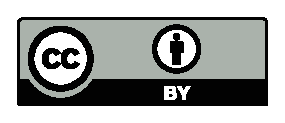
\includegraphics[width=35mm]{common-creatives-by.eps}\hskip5mm
\raise 9mm\hbox{\vtop{\hsize 110mm\noindent
This manual is licensed under the
\hfil\break Creative Commons Attribution 4.0 International License :
\hfil\break{\tt https://creativecommons.org/licenses/by/4.0/}}}

\vfil\eject
\eject

%%%%%%%%%%%%%%%%%%%%%%%%%%%%%%%%%%%%%%%%%%%%%%%%%%%%%%%%%%%%%%%%%%%%%%%%%%%%%%%%%%%%%%%%%%%%%%%
%%%%%%%%%%%%%%%%%%%%%%%%%%%%%%%%%%%%%%%%%%%%%%%%%%%%%%%%%%%%%%%%%%%%%%%%%%%%%%%%%%%%%%%%%%%%%%%

% \bigskip\line{\parfont #1\hfil}\medskip}
\paragraph{Table of contents}

\bigskip\noindent
\numb section 1. General description

\numb section 1.\numb parag 1. An elementary example

\numb section 1.\numb parag 2. Cells and meshes

\numb section 1.\numb parag 3. Joining meshes

\numb section 1.\numb parag 4. Triangular meshes

\numb section 1.\numb parag 5. Mixing triangles and rectangles

\numb section 1.\numb parag 6. Functions


\medskip\noindent
\numb section 2. Meshes and manifolds

\numb section 2.\numb parag 1. Joining segments

\numb section 2.\numb parag 2. Triangular meshes on rectangles

\numb section 2.\numb parag 3. A manifold defined as a level set in $ \RR^2 $

\numb section 2.\numb parag 4. A circle defined by four curved segments

\numb section 2.\numb parag 5. A hemisphere defined by four curved triangles

\numb section 2.\numb parag 6. A more complex surface

\numb section 2.\numb parag 7. Exercise

\numb section 2.\numb parag 8. Alternating between manifolds

\numb section 2.\numb parag 9. Alternating between manifolds, again

\numb section 2.\numb parag 10. An organic shape

\numb section 2.\numb parag 11. A manifold defined by two equations

\numb section 2.\numb parag 12. A submanifold of a submanifold

\numb section 2.\numb parag 13. Parametric manifolds -- a curve

\numb section 2.\numb parag 14. Closing a circle

\numb section 2.\numb parag 15. Parametric manifolds -- a surface

\numb section 2.\numb parag 16. Starting with a high-dimensional manifold


\medskip\noindent
\numb section 3. Progressive mesh generation

\numb section 3.\numb parag 1. Filling a disk

\numb section 3.\numb parag 2. Meshing a circle

\numb section 3.\numb parag 3. Inner boundaries

\numb section 3.\numb parag 4. Meshing a three-dimensional loop

\numb section 3.\numb parag 5. Starting and stopping points

\numb section 3.\numb parag 6. Meshing a compact surface

\numb section 3.\numb parag 7. A more complicated surface

\numb section 3.\numb parag 9. A bumpy hemisphere

\numb section 3.\numb parag 10. How the orientation is chosen

\numb section 3.\numb parag 12. Specifying the direction

\numb section 3.\numb parag 13. The intrinsic and inherent orientations

\numb section 3.\numb parag 14. Revisiting the bumpy hemisphere

\numb section 3.\numb parag 15. Specifying the direction

\numb section 3.\numb parag 16. Geometric limitations

\numb section 3.\numb parag 17. Sharp angles

\numb section 3.\numb parag 18. Sharp edges

\numb section 3.\numb parag 19. Sharp edges, again

\numb section 3.\numb parag 20.
\special{ps: gsave 0.6 setgray}Singularities\special{ps: grestore}

\numb section 3.\numb parag 21.
\special{ps: gsave 0.6 setgray}Singularities, again\special{ps: grestore}

\numb section 3.\numb parag 22. Non-uniform meshing

\numb section 3.\numb parag 23. 
\special{ps: gsave 0.6 setgray}Changing the Riemann metric\special{ps: grestore}

\numb section 3.\numb parag 24. 
\special{ps: gsave 0.6 setgray}Anisotropic metric\special{ps: grestore}

\numb section 3.\numb parag 25. Future work

\medskip\noindent
\numb section 4. \special{ps: gsave 0.6 setgray}Meshing of three-dimensional domains\special{ps: grestore}

\medskip\noindent
\numb section 5. Fields, functions and variational formulations

\numb section 5.\numb parag 1. Fields and functions

\numb section 5.\numb parag 2. \special{ps: gsave 0.6 setgray}Fields and functions\special{ps: grestore} [outdated]


\medskip\noindent
\numb section 6. Finite elements and integrators

\numb section 6.\numb parag 1. Finite elements

\numb section 6.\numb parag 2. A rudimentary example


\medskip\noindent
\numb section 7. \special{ps: gsave 0.6 setgray}Periodicity, quotient manifolds\special{ps: grestore}

\numb section 7.\numb parag 1. \special{ps: gsave 0.6 setgray}A one-dimensional circle\special{ps: grestore}

\numb section 7.\numb parag 2. \special{ps: gsave 0.6 setgray}A flat torus\special{ps: grestore}

\numb section 7.\numb parag 3. \special{ps: gsave 0.6 setgray}A skew flat torus\special{ps: grestore}

\numb section 7.\numb parag 4. \special{ps: gsave 0.6 setgray}A curved circle\special{ps: grestore}

\numb section 7.\numb parag 5. \special{ps: gsave 0.6 setgray}A cylinder\special{ps: grestore}

\numb section 7.\numb parag 6. \special{ps: gsave 0.6 setgray}A curved torus\special{ps: grestore}


\medskip\noindent
\numb section 8. A closer look at cells and meshes

\numb section 8.\numb parag 1. Building cells and meshes

\numb section 8.\numb parag 2. A ring-shaped mesh

\numb section 8.\numb parag 3. Lists of cells inside a mesh

\numb section 8.\numb parag 5. Iterators over cells

\numb section 8.\numb parag 6. Iterators over chains of segments

\numb section 8.\numb parag 7. Orientation of cells inside a mesh

\numb section 8.\numb parag 8. Navigating inside a mesh

\numb section 8.\numb parag 9. Navigating at the boundary of a mesh

\numb section 8.\numb parag 10. Declaring cells and meshes


\medskip\noindent
\numb section 9. More on manifolds

\numb section 9.\numb parag 1. Projecting points on an implicit manifold


\medskip\noindent
\numb section 10. Technical details

\numb section 10.\numb parag 1. Namespaces and class names

\numb section 10.\numb parag 2. Tags

\numb section 10.\numb parag 3. Wrappers and cores

\numb section 10.\numb parag 4. The lifecycle of objects

\numb section 10.\numb parag 5. \special{ps: gsave 0.6 setgray}Different kinds of meshes\special{ps: grestore}

\numb section 10.\numb parag 6. Maximum topological dimension

\numb section 10.\numb parag 7. Declaring cell cores

\numb section 10.\numb parag 8. Disposing of meshes

\numb section 10.\numb parag 9.
\special{ps: gsave 0.6 setgray}About {\tt init\_cell}\special{ps: grestore}

\numb section 10.\numb parag 11. Programming style

\numb section 10.\numb parag 12. Frequent errors at compile time

\numb section 10.\numb parag 13. Frequent errors at run time

\numb section 10.\numb parag 15. Chains of segments

\numb section 10.\numb parag 16. The cloud

\numb section 10.\numb parag 17. The cloud in progressive mesh generation


\medskip\noindent
\numb section 11. Internal details

\numb section 11.\numb parag 2. Building a chain of segments

\numb section 11.\numb parag 3. Building a rectangular mesh

\numb section 11.\numb parag 4. Building a triangular mesh

\numb section 11.\numb parag 5. Progressive mesh generation

\numb section 11.\numb parag 6. The normals

\numb section 11.\numb parag 7. Filling triangles

\numb section 11.\numb parag 8. Touching the interface

\medskip\noindent
Index


 \input manual-cap-01
% \input manual-cap-02
% \input manual-cap-03
% \input manual-cap-04
% \input manual-cap-05
% \input manual-cap-06
% \input manual-cap-07
% \input manual-cap-08
% \input manual-cap-09
% \input manual-cap-10
% \input manual-cap-11



\section{Index}

boundary of a cell : \numb section 1.\numb parag 2, \numb section 8.\numb parag 3

cell : \numb section 1.\numb parag 2, \numb section 8.\numb parag 1

cloud : see {\codett MetricTree}

compilation process : \numb section 10.\numb parag 13

dimension of a cell or mesh : \numb section 1.\numb parag 2, \numb section 10.\numb parag 3,
\numb section 10.\numb parag 6

discarding a mesh : \numb section 10.\numb parag 8

docking (of a finite element on a cell) : \numb section 6.\numb parag 1

errors : \numb section 10.\numb parag 12, \numb section 10.\numb parag 13

{\codett Field} : \numb section 5.\numb parag 1

finite element : section \numb section 6

{\codett Function} : \numb section 1.\numb parag 6, \numb section 5.\numb parag 1

interpolation of coordinates : \numb section 2.\numb parag 3 -- \numb section 2.\numb parag 9,
\numb section 11.\numb parag 2 -- \numb section 11.\numb parag 4

iterators over cells : \numb section 8.\numb parag 5, \numb section 8.\numb parag 7

{\codett init\_cell} : \numb section 10.\numb parag 9

{\codett join}ing meshes : \numb section 1.\numb parag 3, \numb section 1.\numb parag 4,
\numb section 1.\numb parag 5, \numb section 2.\numb parag 1, \numb section 2.\numb parag 2,
\numb section 2.\numb parag 4, \numb section 2.\numb parag 5, \numb section 2.\numb parag 6,
\numb section 8.\numb parag 2

level set : see manifold, defined by an implicit equation

m-tree : \numb section 10.\numb parag 16

manifold, Euclidian : all over the place\hfil\break
\hglue 15mm (any code using {\maniFEM} must begin by declaring a Euclidian manifold)

manifold, defined by an implicit equation : \numb section 2.\numb parag 4 --
\numb section 2.\numb parag 9, section \numb section 3

manifold, parametric : \numb section 2.\numb parag 13, \numb section 2.\numb parag 14

manifold, quotient : section \numb section 7

mesh : all over the place, esp.\ \numb section 1.\numb parag 2, \numb section 1.\numb parag 3,
\numb section 8.\numb parag 1, \numb section 8.\numb parag 3, \numb section 8.\numb parag 7
-- \numb section 8.\numb parag 10

{\codett MetricTree} : \numb section 10.\numb parag 16, \numb section 10.\numb parag 17

negative {\codett Cell} or {\codett Mesh} : see orientation of {\codett Cell}s and
{\codett Mesh}es

oct-tree : \numb section 10.\numb parag 16

orientation of {\codett Cell}s and {\codett Mesh}es : \numb section 1.\numb parag 2,
\numb section 1.\numb parag 3, \numb section 8.\numb parag 1, \numb section 8.\numb parag 7,
\numb section 10.\numb parag 7

orientation of a {\codett Manifold} : \numb section 3.\numb parag 10

parametric manifold : see manifold, parametric

progressive mesh generation : section \numb section 3, \numb section 10.\numb parag 17,
\numb section 11.\numb parag 5 -- \numb section 11.\numb parag 8

projection, onto a manifold : \numb section 2.\numb parag 3 -- \numb section 2.\numb parag 9

quad-tree : \numb section 10.\numb parag 16

quotient manifold : see manifold, quotient

reverse cell or mesh : see orientation of cells and meshes

segment {\codett Cell}s : \numb section 1.\numb parag 2

segment {\codett Mesh}es : \numb section 1.\numb parag 1 -- \numb section 1.\numb parag 3,
\numb section 10.\numb parag 15

{\codett set\_as\_working\_manifold} : \numb section 2.\numb parag 8 --
\numb section 2.\numb parag 10, \numb section 2.\numb parag 12, \numb section 3.\numb parag 1,
\numb section 3.\numb parag 2, \numb section 3.\numb parag 3, \numb section 3.\numb parag 9,
\numb section 3.\numb parag 14 -- \numb section 3.\numb parag 24

{\codett tag}s : \numb section 10.\numb parag 2

wrapper : \numb section 8.\numb parag 1, \numb section 8.\numb parag 10, \numb section 10.\numb parag 3


\bye



%%%%%%%%%%%%%%%%%%%%%%%%%%%%%%%%%%%%%%%%%%%%%%%%%%%%%%%%%%%%%%%%%%%%%%%%%%%%%%%%%%%%%%%%%%%%%%%

\hbox{\includegraphics[width=19mm]{manifem-small.eps}}


The factory function {\codett FE\_function::from\_string} accepts expressions like {\codett "x+y+z"} or
{\codett "x\^{}3-.22E-4*y\^{}2+5.4"} (which stands for $ x^3 - 0.0000022y^2+5.4$) 
but not expressions involving parentheses.

There are other ways of building symbolic expressions.
For example,

\verbatim
   auto fx = FE_function::from_string ( "x" ); // FE_function * fx
   auto fy = FE_function::from_string ( "y" );
   auto five = FE_function::constant (5); // FE_function * five
   auto s = FE_function::sum (fx,fy,five); // FE_function * s
   auto p = FE_function::power (s,3); // FE_function * p, or
   // p = (x+y+5)^3
\endverbatim

\noindent or

\verbatim
double ff(double x, double y) { return sin(x)*cos(y); }
int main () {
   auto f = FE_function::function (ff); // FE_function * f
}\endverbatim















